% ============================ INTRODUCTION ============================
Tracked and wheeled robots cannot ascend an obstacle taller than their leading wheel.
\emph{Articulated} tracked robots address higher obstacles with flippers,
independently actuated sub-tracks that reshape the robot's morphology on the fly: they
can be used to reach beyond the leading wheel to ascend what tracked and wheeled robots cannot, and to
free the robot when it gets \emph{stuck}~\cite{yuan2019,chen2023,xu2024}.



\begin{figure}[t]
  \centering
  \begin{tikzpicture}[inner sep=0, outer sep=0]
    \node[anchor=north west] (ra) at (0,0)
      {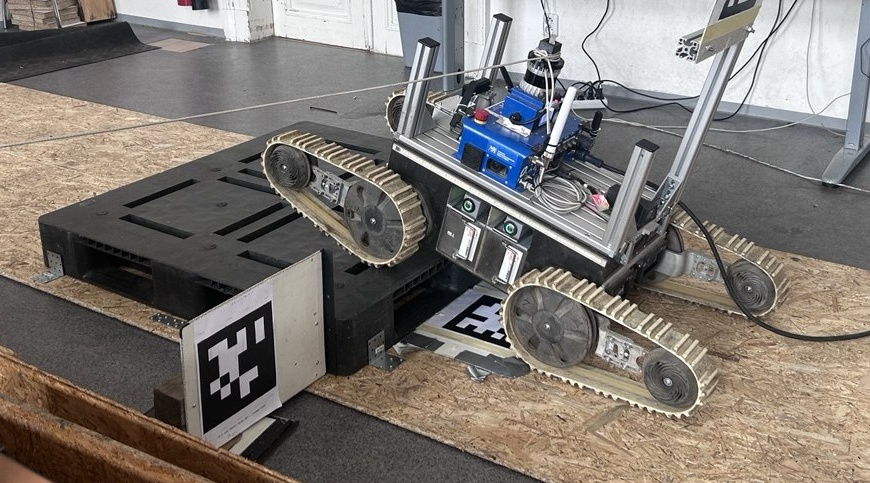
\includegraphics[width=\linewidth]{figures/real_robot_crop.jpg}};
    \node[anchor=north west] (rb) at (ra.south west)
      {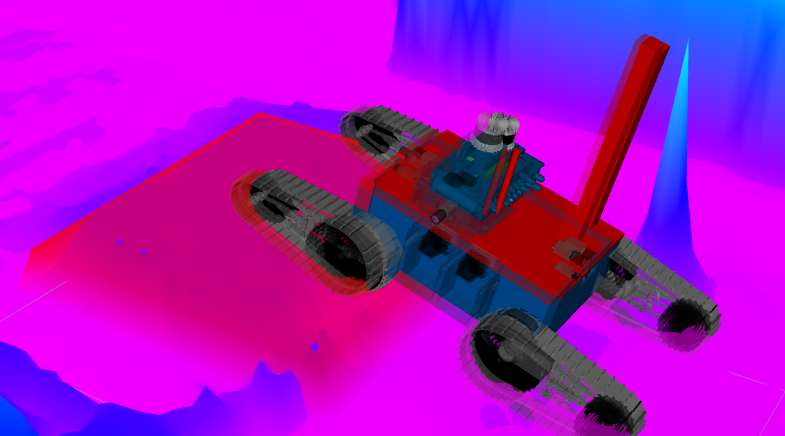
\includegraphics[width=\linewidth]{figures/simulated_robot_crop.png}};
    \node[anchor=north west, inner sep=1.5pt, fill=white, fill opacity=0.75,
          text opacity=1, font=\bfseries\small] at (ra.north west) {(a)};
    \node[anchor=north west, inner sep=1.5pt, fill=white, fill opacity=0.75,
          text opacity=1, font=\bfseries\small] at (rb.north west) {(b)};
  \end{tikzpicture}
  \caption{\textbf{The onboard map against ground truth on a pallet.} (a) The robot climbing a
  pallet obstacle. (b) The same pose, rendered from the data the robot observed there: the
  onboard map (blue) against the handcrafted ground-truth
  map positioned by AprilTags (transparent red), with the ground-truth robot pose drawn
  transparent. The offset between the two surfaces, and between the two bodies, is the map and localization error that the perception stack introduces. The spike behind the robot in the onboard map is a reflected, invalid LiDAR return.}
  \label{fig:robot}
\end{figure}

\textbf{Prior flipper controllers assume an elevation map.}
Across the literature, semi-autonomous and autonomous flipper controllers share a
precondition: they consume an \emph{elevation map} of the terrain under and in front of the
robot as their dominant
input~\cite{chen2023,oehler2024,yuan2019,xu2024,pan2023icm,pan2023atd3qn,ctrac2025,azayev2022}.
Fully manual teleoperation needs no map because the operator sees the terrain from a
third-person view, but must drive all four flippers by hand. 

\textbf{On a real robot, the map is a dead-reckoning artifact.}
Where the estimate of that terrain drifts, due to body occlusion, the commanded flipper
angles are computed for incorrect terrain. Onboard sensors
observe what is ahead, but the body occludes their view of the terrain beneath it.
Dedicated underbody sensors could measure it, but they are rarely fitted and have very
low resolution. That terrain can therefore mainly be \emph{remembered}: observed earlier, accumulated into an elevation
map, and carried beneath the robot as it advances by
\emph{integrating wheel or LiDAR odometry}~\cite{fankhauser2018}. Every stage of this
pipeline is a dead-reckoning process: point-cloud deskewing warps each scan by the estimated
sensor trajectory, and elevation mapping registers successive scans through the
estimated motion~\cite{loam2014}. On the loose, deformable,
step-like terrain where flippers are needed, odometry is least reliable: tracks slip, and
the chassis pitches and drops abruptly, saturating the IMU, and inertial integration cannot
recover the estimate either~\cite{woodman2007imu}. Reflected, invalid LiDAR returns add obstacles that do
not exist, such as the spike behind the robot in Fig.~\ref{fig:robot}.

\textbf{The hardest case is a hidden obstacle.}
When a rigid obstacle is \emph{hidden} (Fig.~\ref{fig:grass}), optical sensors, such as LiDAR or cameras, return the
compliant canopy above it, while the load-bearing obstacle beneath remains invisible until the
chassis stalls on it. Neither a dedicated underbody sensor, which is blinded by the same vegetation, nor foliage-penetrating radar, which is bulky and low-resolution, resolves this in practice.

\textbf{Our contribution: control of the flippers without a map and without an accumulated
pose.}
We present \emph{Stabilizing Anti-Stuck} (\SAS), a reactive controller that requires no
elevation map. It has two terms: a
stabilization term that stabilizes the robot body regardless of the terrain, whether
climbing or descending an obstacle, and an anti-stuck term that frees the robot when it
gets stuck by driving the flippers down. To tell a stuck robot from a moving one, the
anti-stuck term needs a motion cue: a thresholded answer to whether the robot is
moving, which requires neither an accurate nor a metric estimate of the motion. Because the
cue is computed over a short window and is never accumulated, \SAS{} never inherits the drift that corrupts the map. 


\needspace{5\baselineskip}%
\textbf{Contributions:}
\nopagebreak
\begin{enumerate}
  \item We propose \SAS, a mapless flipper controller that needs only a
  thresholded motion cue, combining continuous roll and pitch stabilization with a reactive
  anti-stuck term under a safe directional-priority blend.
  \item We measure the degradation of the elevation map caused by body occlusion and
  odometry drift by evaluating map-based baselines under both a \emph{ground-truth} map and
  the \emph{onboard} map, in a large comparison in simulation of \SAS{} against \emph{twelve}
  map-based baselines and two manual baselines on a twelve-obstacle course; every controller
  drives the full course ten times, with the perception stack reset at each obstacle.
  \item We perform the large comparison on a real obstacle arena with AprilTag ground
  truth: on a four-track robot, each controller drives ten times over a pallet obstacle.
\end{enumerate}
